\documentclass[10pt,handout,english]{beamer}
\usetheme{Warsaw}
\usepackage{graphicx}
\usepackage{placeins}
\usepackage{amsmath}
\usepackage{tabu}
\usepackage{bbm}
\usepackage{booktabs}
\usepackage[round]{natbib}
\usepackage{bm}
\usepackage{ragged2e}
\usepackage{hyperref}
\usepackage{amsmath}
\usepackage{xcolor}
\usepackage[super]{nth}
\hypersetup{
    colorlinks=true,
    linkcolor=blue,
    filecolor=blue,      
    urlcolor=blue,
    citecolor=black,
}

\apptocmd{\frame}{}{\justifying}{} % Allow optional arguments after frame.

\setbeamertemplate{frametitle continuation}{}

\newcommand\setItemnumber[1]{\setcounter{enumi}{\numexpr#1-1\relax}}

\newcommand{\ts}{\textsuperscript}
\newcommand{\E}{\mathbb{E}}
\newcommand{\R}{\mathbb{R}}
\newcommand{\F}{\mathcal{F}}
\newcommand{\1}{\mathbbm{1}}

\title[]{Classical versus high-dimensional theory}
\author[Kaveh S. Nobari]{Kaveh S. Nobari}
\institute[]{Reading Sessions in High-Dimensional Statistics}
\date[27/10/2020]
{Department of Mathematics and Statistics\\ Lancaster University}
	

\begin{document}
\begin{frame}
\titlepage
\end{frame}


\begin{frame}{Contents}
\tableofcontents
\end{frame}

\section{Classical vs high-dimensional framework}
\frame{\tableofcontents[currentsection]}
\begin{frame}{Classical framework}
\begin{itemize}
\item{} Classical theory provides statement for a fixed class of models, parameterised by an index $n$ (interpreted as sample size) that is allowed to increase.\justifying
{\vskip 0.5em}
\item{} An instance of the earlier statement is the simplest setup of the \textcolor{red}{law of large numbers}: given restrictions on dependence, heterogeneity, and moments of sequence of random variables $\{X_i\}_{i=1}^n$, $\bar{X}_n-\mu\overset{a.s.}{\to}0$, where $\bar{X}_n\equiv n^{-1}\sum\limits_{i=1}^{n}X_i$ and $\mu=\E[X_n]$ [see \citet{white2014asymptotic}]. Consequently, the sample mean $\bar{X}_n$ is a consistent estimator of the unknown population mean.\justifying
{\vskip 0.5em} 
\item{} A more refined statement is provided by the \textcolor{red}{central limit theorem} that guarantees the rescaled deviation $\sqrt{n}(\bar{X}_n- \mu)$ converges in distribution to a Gaussian distribution with zero mean and covariance matrix $\Sigma$. \justifying
{\vskip 0.5em}
\item{} In classical framework, the dimension $d$ of the data space is typically \textcolor{red}{fixed}, while $d\to\infty$.\justifying
\end{itemize}
\end{frame}

\begin{frame}{High-dimensional framework}
\begin{itemize}
\item{} In a high-dimensional framework, the dimension $d$ is either of the \textcolor{red}{same order} as the sample size $n$ - i.e. $d\asymp n$ or the degree of dimensionality is \textcolor{red}{much larger} than the sample size - i.e. $d\gg n$.\justifying
{\vskip 0.5em}
\item{} In such framework, the classical large $n$, fixed $d$ theory \textcolor{red}{fails to provide useful predictions.}\justifying
{\vskip 0.5em}
\item{} Classical methods can break down dramatically in high-dimensional regimes.\justifying
{\vskip 0.5em}
\item{} In this session, we follow chapter 1 of \citet{wainwright2019high} to motivate the study of high-dimensional statistics.\justifying  
\end{itemize}
\end{frame}
\section{What can go wrong in high dimensions?}
\frame{\tableofcontents[currentsection]}
\begin{frame}[allowframebreaks]{Example: linear discriminant analysis}
\begin{itemize}
\item{} Suppose we wish to determine whether an observation vector $x\in \R^d$ has been drawn from one of two possible distributions, say $P_1$ v.s. $P_2$.\justifying
{\vskip 0.5em}
\item{} When the two distributions are known, then a natural decision rule is based on thresholding the log-likelihood ratio\justifying   
\[
\psi(x)=\log\frac{P_2[X]}{P_1[X]}
\]
where we reject the null hypothesis that $x$ comes from the distribution $P_1[x]$ when\justifying
\[
\psi(x)>c
\]
such that $c$ is the smallest constant that satisfies $P[TS>c]\leq \alpha$, for $0\leq \alpha\leq 1$, where $\alpha$ is an arbitrary significance level.\justifying
{\vskip 0.5em}
\item{} The Neyman-Pearson Lemma guarantees that these family of decision rules are optimal (maximize power for a given testing problem).\justifying
\end{itemize}
{\vskip 0.5em}
Now suppose $P_1$ and $P_2$ are distributed as multivariate Gaussian, say $N(\mu_1,\Sigma)$ and $N(\mu_2,\Sigma)$, with differing only in their mean vectors. Furthermore recall, that for a multivariate Gaussian random variable, the density $P_i[X]$ for $i=1,2$ is defined as follows\justifying
\[
P_i[x]=\frac{1}{(2\pi)^{d/2}\lvert\Sigma\rvert^{1/2}}\exp\left(-\frac{1}{2}(x-\mu_i)'\Sigma^{-1}(x-\mu_i)\right)
\]
therefore, 
\begin{align*}
\psi(x)&=\log\frac{P_2[X]}{P_1[X]}\\
&=\left\{\frac{1}{2}(x-\mu_1)'\Sigma^{-1}(x-\mu_1)-\frac{1}{2}(x-\mu_2)'\Sigma^{-1}(x-\mu_2)\right\}
\end{align*}
Noting that $B(x,y):=\frac{1}{2}x'\Sigma^{-1}y$ is a symmetric bilinear form, we have\justifying
\begingroup
\allowdisplaybreaks
\begin{align*}
\psi(x)&=\log\frac{P_2[X]}{P_1[X]}\\
&=B(x-\mu_1,x-\mu_1)-B(x-\mu_2,x-\mu_2)\\
&=B(x,x)-B(x,\mu_1)-B(\mu_1,x)+B(\mu_1,\mu_1)\\
&\textcolor{white}{=}-B(x,x)+B(x,\mu_2)+B(\mu_2,x)-B(\mu_2,\mu_2)\\
&=2B(x,\mu_2)-2B(x,\mu_1)+B(\mu_1,\mu_1)-B(\mu_2,\mu_2)\\
&=2B(x,\mu_2-\mu_1)+B(\mu_1-\mu_2,\mu_1+\mu_2)\\
&=2B(x,\mu_2-\mu_1)-B(\mu_2-\mu_1,\mu_2+\mu_1)\\
&=x'\Sigma^{-1}(\mu_2-\mu_1)-\frac{1}{2}(\mu_2-\mu_1)'\Sigma^{-1}(\mu_2+\mu_1)
\end{align*}
\endgroup
The earlier results reduces to the linear test statistic\justifying 
\[
\psi(x):=\left\langle\mu_1-\mu_2,\Sigma^{-1}\left(x-\frac{\mu_1+\mu_2}{2}\right)\right\rangle
\]
where $<.,.>$ denotes the Euclidean inner product in $\R^d$.\justifying

\begin{itemize}
\item{} The optimal decision rule is based of thresholding $\psi(x)$, where the quality of the decision is obtained by computing the optimal probability of incorrect classification. For an example of incorrect classification, refer to the plot below that has been extracted from \citet{johnson2002applied}\justifying 
{\vskip 0.5em}
\end{itemize}
\end{frame}
\begin{frame}
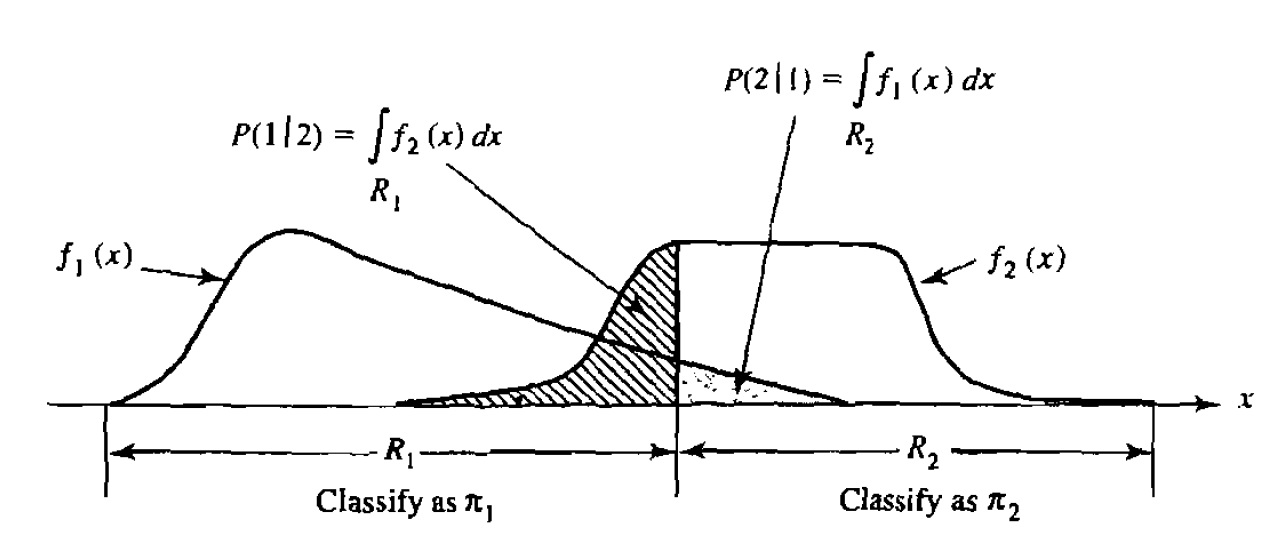
\includegraphics[width=\textwidth]{Classif}
\end{frame}
\begin{frame}[allowframebreaks]
\begin{itemize}
\item{} If two classes are equally likely, the probability is given by\justifying 
\[
Err(\psi)=\frac{1}{2}\left\{P_1[\psi(X')\leq0]+P_2[\psi(X'')>0]\right\}
\]  
where $X'$ and $X''$ are random vectors drawn from the distributions $P_1$ and $P_2$ respectively. Given the Gaussian assumption, the error probability can be expressed as\justifying 
\begin{align*}
Err[\psi]&=\frac{1}{\sqrt{2\pi}}\int_{-\infty}^{-\gamma/2}\exp\left(\frac{-t^2}{2}\right)dt\\
&=\Phi\left(\frac{-\gamma}{2}\right)
\end{align*}
where $\Phi$ is the Gaussian CDF and where
\[
\gamma=\sqrt{(\mu_1-\mu_2)'\Sigma^{-1}(\mu_1-\mu_2)}
\]
{\vskip 0.5em}
\item{} Assuming a Gaussian distribution and two labelled samples $\{x_i\}_{i=1}^{n_1}$ and $\{x_i\}_{i=n_1+1}^{n_2}$ which are drawn independently from $P_1$ and $P_2$, we may estimate the parameters of the log-likelihood ratio using their empirical counterparts, namely the sample mean $\hat{\mu}$ and the sample covariance matrix $\hat{\Sigma}$.\justifying 
{\vskip 0.5em}
\item{} Substituting these estimates in the log-likelihood ratio yields\justifying 
\[
\hat{\psi}(x):=\left\langle\hat{\mu}_1-\hat{\mu}_2,\hat{\Sigma}^{-1}\left(x-\frac{\hat{\mu}_1+\hat{\mu}_2}{2}\right)\right\rangle
\]
\item{} Let us assume that the two classes are equally likely, the error probability by using a zero threshold is given by\justifying 
\[
Err[\hat{\psi}]=\frac{1}{2}\left\{P_1[\hat{\psi}(X')\leq0]+P_2[\hat{\psi}(X'')>0]\right\}
\]
\item{} Let us now assume that the covariance matrix $\Sigma$ is known a priori and is assumed to be the identity matrix, leading to the test statistic\justifying 
\[
\hat{\psi}(x):=\left\langle\hat{\mu}_1-\hat{\mu}_2,x-\frac{\hat{\mu}_1+\hat{\mu}_2}{2}\right\rangle
\]
\item{} Kolmogorov showed that in high-dimensional asymptotic framework, in which $(n_1,n_2,d)\to\infty$ and with $d/n_i\to\alpha>0$ for $i=1,2$ and the Euclidean distance $\lVert \mu_1-\mu_2 \rVert_2^2\to \gamma>0$, the error probability\justifying  
\[
Err[\hat{\psi}]\overset{p}{\to}\Phi\left(-\frac{\gamma^2}{2\sqrt{\gamma^2+2\alpha}}\right)
\] 
\item{} \textbf{Question:} What happens when $d/n_i\to 0$? What about when $d/n_i\to \alpha>0$?\justifying 
\end{itemize}
\end{frame}

\begin{frame}{Classical vs high-dimensional error rate}
In the classical setting, the asymptotic error probability was given by\justifying 
\[
Err[\hat{\psi}]=\Phi\left(-\frac{\gamma}{2}\right)
\]
with its high-dimensional analogue being
\[
Err[\hat{\psi}]\overset{p}{\to}\Phi\left(-\frac{\gamma^2}{2\sqrt{\gamma^2+2\alpha}}\right)
\]
Looking at the following plots, is the error probability better described by the classical or high-dimensional theory?
\end{frame}
\begin{frame}
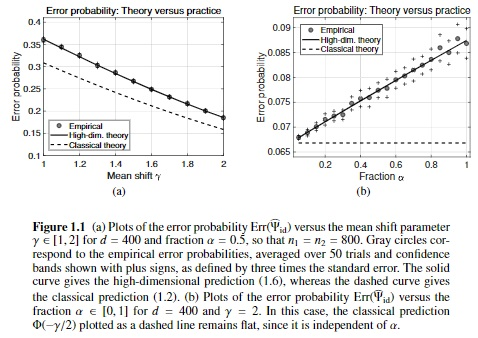
\includegraphics{ErrPerf}
\end{frame}
\section{What can help us in high dimensions?}
\frame{\tableofcontents[currentsection]}
\begin{frame}
\begin{itemize}
\item{} High-dimensional phenomena outlined in many settings are \textcolor{red}{unavoidable}.
{\vskip 0.5em}
\item{} In the classification problem earlier, if $d/n_i>0$ it is impossible obtain optimal classification rate. 
{\vskip 0.5em}
\item{} Hope is that the data harbours some form of a \textcolor{red}{low-dimensional structure}.
\end{itemize}
\end{frame}

\section{What is the non-asymptotic view}
\frame{\tableofcontents[currentsection]}
\begin{frame}
\begin{itemize}
\item{} \textcolor{red}{Classical asymptotics:} $n\to\infty$ while other problem parameters remain fixed.
{\vskip 0.5em}
\item{}\textcolor{red}{High-dimensional asymptotics:} $(n,d)\to\infty$, while enforcing that for some scaling function $\Psi$, the sequence $\Psi(n,d)$ remains fixed or $\Psi(n,d)\to\alpha\in[0,\infty)$. The scaling function $\Psi$ may be as simple $\Psi(n,d)=d/n$, as shown earlier, or it may use other parameters, such as the sparsity parameter $s$ [provide example].
{\vskip 0.5em}
\item{}\textcolor{red}{Non-asymptotic bounds:} $(n,d)$ as well as other parameters are viewed as fixed and high probability statements are made as a function of them. 
\end{itemize}
{\vskip 0.5em}
\textbf{Conclusion:} The knowledge of tail bounds and concentration inequalities is crucial for assessing the performance of statistical estimators.
\end{frame}

\begin{frame}[allowframebreaks]
\frametitle{References}
\bibliographystyle{apa}
\bibliography{References_HDStat}
\end{frame}
\end{document}